\documentclass[a4paper,12pt]{article}

\usepackage[utf8]{inputenc}
\usepackage[spanish]{babel}
\usepackage{geometry}
\usepackage{titlesec}
\usepackage{enumitem}
\usepackage{tocloft}
\usepackage{hyperref}
\usepackage{tabularx}
\usepackage{lipsum}
\usepackage{fancyhdr}
\usepackage{graphicx}
\usepackage{float}
\usepackage{titlesec}
\usepackage{tocloft}
\usepackage{caption}
\usepackage{datetime}
\newdateformat{monthyeardate}{\monthname[\THEMONTH], \THEYEAR}
\DeclareUnicodeCharacter{0301}{\'{e}}
\titleformat*{\section}{\LARGE\bfseries}

\usepackage[backend=biber, style=ieee]{biblatex}
\addbibresource{references/ref.bib}



\setcounter{secnumdepth}{4} % Numeración hasta el nivel de subsubsección
\setcounter{tocdepth}{4} % Inclusión en la tabla de contenidos hasta el nivel de subsubsección


\geometry{margin=2.5cm}

%\titleformat{\section}[block]{\normalfont\bfseries}{\thesection}{1em}{}
\titlespacing*{\section}{0pt}{\baselineskip}{\baselineskip}




\renewcommand{\cftsecleader}{\cftdotfill{\cftdotsep}}

% Configuración de fancyhdr para pie de página y encabezado
\pagestyle{fancy}
\fancyhf{}  % Limpiar estilos anteriores
\chead{\bfseries PLAN DE TRABAJO DE GRADO}  % Encabezado centrado
\rhead{\monthyeardate\today}  % Encabezado en la derecha
\cfoot{Universidad Industrial de Santander}  % Pie de página central
\rfoot{\thepage}  % Número de página en la derecha
\renewcommand{\headrulewidth}{1pt}  % Línea en el encabezado
\renewcommand{\footrulewidth}{1pt}  % Línea en el pie de página


\begin{document}

\begin{titlepage}
    \begin{center}
        {\fontsize{14}{14}\selectfont UNIVERSIDAD INDUSTRIAL DE SANTANDER \par}
        \vspace{10pt}
        {\fontsize{14}{14}\selectfont FACULTAD DE INGENIERÍAS FISICOMECÁNICAS \par}
        \vspace{10pt}
        {\fontsize{14}{14}\selectfont ESCUELA DE INGENIERÍA DE SISTEMAS E INFORMÁTICA \par}
        \vspace{10pt}
        \vspace{10pt}
        \vspace{10pt}
        \vspace{10pt}
        \vspace{10pt}
        {\fontsize{14}{14}\selectfont PLAN DE TRABAJO DE GRADO \par}
        \vspace{10pt}
        \vspace{10pt}
        \vspace{10pt}
        \vspace{10pt}
    \end{center}
    {\normalsize \textbf{FECHA DE PRESENTACIÓN:} Bucaramanga, \today \par}
    \vspace{1cm}
    {\normalsize \textbf{TITULO:} Prototipo de sistema de observabilidad de microservicios backend para el proyecto de Renovación de los Sistemas de Información UIS (R.S.I). \par}
    \vspace{1cm}
    {\normalsize \textbf{MODALIDAD:} Proyecto de investigación \par}
    \vspace{1cm}
    {\normalsize \textbf{AUTOR:} Camilo Ciro Orozco - 2190055, Amin Esteban Barbosa Vargas - 2190037 \par}
    \vspace{1cm}
    {\normalsize \textbf{DIRECTOR:} Emilio Justiniano Carcamo Troconis, Escuela de Ingeniería de Sistemas e Informática. \par}
    \vspace{1cm}
    {\normalsize \textbf{ENTIDAD INTERESADA:} Universidad Industrial de Santander. \par}
\end{titlepage}

\tableofcontents

\newpage

\begin{center}
\large DISEÑO DE SISTEMA DE OBSERVABILIDAD PARA LOS MICROSERVICIOS BACKEND EN EL PROYECTO DE RENOVACIÓN DE LOS SISTEMAS DE INFORMACIÓN UIS (R.S.I.)
\end{center}

%%%%%%%%%%%%%%%%%%%%%%%%%%%%
%%%%%%%%%%%%%%%%%%%%%%%%%%%%    INTRODUCCION
%%%%%%%%%%%%%%%%%%%%%%%%%%%%
\section{\large INTRODUCCIÓN}
\vspace{12pt}

La arquitectura de microservicios consta de una colección de servicios autónomos y pequeños que permite manejar diferentes lógicas empresariales para solucionar requerimientos especı́ficos donde cada uno de ellos realiza sus propias pruebas, gestiona sus dependencias y demás implementaciones relacionadas a su correcto funcionamiento, permitiendo ası́ partir de pequeñas tareas a la integración de un conjunto global; de esta manera ya se tiene una aplicación escalable y flexible a cualquier tipo de cambio que se requiera. Sin embargo, si bien es cierto que con este tipo de modelos tenemos mayor control de nuestro sistema, se suele tener el problema de crear y usar microservicios de forma descontrolada, ocasionando que la complejidad del sistema también crezca y a su vez, hace más difı́cil mantener una depuración estable para cada uno de ellos, por ese motivo, se emplean métodos de monitoreo. Supervisar los sistemas basados en microservicios es una tarea fundamental debido a que nos permite conocer cómo controlarlo, asegurarnos que sea fiable, se encuentre disponible y que funcione como se tiene imaginado.

\vspace{12pt}

En la actualidad, la Universidad Industrial de Santander y su equipo encargado en la Renovación de los Sistemas de Información (RSI) cuentan con un sistema de monitoreo, que teóricamente permite la observación y el análisis de los datos registrados, por cada microservicio, que informa sobre el estado actual de la aplicación. No obstante, se ha realizado una investigación sobre dicho servicio y se ha encontrado que falla en gran medida en su estudio, no diseña las gráficas y/o los informes esperados, además, de ser bastante antiguo. Este es un problema que en gran medida afecta a los desarrolladores encargados del proyecto, después de todo, si un error llegase a ocurrir en el sistema lo ideal sería revisar el informe creado por dicho sistema de supervisión, al no funcionar correctamente, implica recurrir a diferentes métodos para identificar el fallo y eso se refleja principalmente en un mayor gasto de tiempo.

\vspace{12pt}
Es por ese motivo que este proyecto tiene el objetivo de analizar e idear un prototipo para un sistema de observabilidad a nivel de backend en el proyecto de Renovación de los Sistemas de Información (RSI), que satisfaga los 3 pilares fundamentales de la observabilidad: métricas, logs y trazas. Ademas, se realizaran estudios utilizando distintos sistemas de monitoreo que nos permita hallar el mas optimo, sencillo y eficiente para así poder proponer el prototipo ideal.

%%%%%%%%%%%%%%%%%%%%%%%%%%%%
%%%%%%%%%%%%%%%%%%%%%%%%%%%%    PLANTEAMIENTO Y JUSTIFICACION DEL PROBLEMA
%%%%%%%%%%%%%%%%%%%%%%%%%%%%
\section{\large PLANTEAMIENTO Y JUSTIFICACIÓN DEL PROBLEMA}

Actualmente, en la capa backend del proyecto RSI, se emplea una arquitectura basada en microservicios. El proyecto empezó a finales de 2018 y, a la fecha de este documento, cuenta con alrededor de 13 aplicaciones backend donde cada una ofrece múltiples lógicas de negocio implementadas en API RESTful que son esenciales para el correcto funcionamiento de los sistemas de información.

\vspace{12pt}

Es importante destacar que la cantidad de servicios independientes en cada proyecto puede aumentar con el tiempo. Siempre y cuando los servicios estén disponibles y preparados para su uso, tener numerosos microservicios no debería presentar ningún problema. Sin embargo las fallas son habituales en los sistemas informáticos. Cuando se produce un fallo, los servicios involucrados permanecen inoperables hasta que se detecte y se resuelva el problema. Es por lo anterior que la prioridad en este tipo de casos es reducir el lapso de tiempo entre la ocurrencia del fallo y su resolución. 

\vspace{12pt}

Para lo anterior, en RSI se tiene una herramienta propia llamada “Monitor”, que muestra en un gráfico los logs generados por las diferentes aplicaciones desarrolladas en SpringBoot (framework backend utilizado en el proyecto). La herramienta monitor puede resultar útil para errores específicos que se identifican a simple vista a través de los logs, por lo cual podemos afirmar que entra en el concepto de monitoreo, no obstante, dicha herramienta no cuenta con la capacidad de medir y monitorear a fondo los microservicios realizados en el proyecto, por ese motivo, se recomienda un sistema nuevo de Observabilidad. Con el desarrollo de este proyecto, se espera implementar un prototipo que permita el monitoreo de los logs, trazas y métricas generadas por los servicios y la medición del estado interno del sistema para la prevención o identificación de fallos.

\vspace{12pt}

En resumen, la implementación de conceptos de observabilidad mejora las estrategias de escalado de los equipos DevOps, utilizando los datos de telemetría para definir una estrategia y llevar a cabo una planificación de recursos más efectiva.

\vspace{12pt}

Teniendo presente lo anterior, surgen las preguntas de  investigación sobre la observabilidad en microservicios del proyecto de RSI que motivan el desarrollo de este proyecto: ¿Por qué se debería desarrollar el prototipo de un sistema de observabilidad si el proyecto cuenta con uno ya implementado? ¿Con la estructura actual del proyecto, qué modelo o prototipo se adaptaría mejor?


%%%%%%%%%%%%%%%%%%%%%%%%%%%%
%%%%%%%%%%%%%%%%%%%%%%%%%%%%    OBJETIVOS
%%%%%%%%%%%%%%%%%%%%%%%%%%%%
\section{\large OBJETIVOS}
\subsection{\normalsize OBJETIVO GENERAL}
\begin{itemize}
	\item Diseñar un prototipo para un sistema de observabilidad que permita la recolección y visualización de logs, métricas y trazas de los microservicios backend utilizados en el proyecto RSI.
\end{itemize}

\subsection{\normalsize OBJETIVOS ESPECÍFICOS}

\begin{itemize}
    \item Investigar sobre los distintos conceptos que se deben tener en cuenta a la hora de prototipar un sistema de observabilidad. 
    \item Realizar un estudio preliminar sobre la  infraestructura actual del proyecto de RSI.
    \item Identificar las métricas que sean de gran importancia conocer para una infraestructura como la de RSI.
    \item Hacer una revisión de herramientas para el monitoreo de microservicios y seleccionar las que mejor se adapten al proyecto RSI.
\end{itemize}


%%%%%%%%%%%%%%%%%%%%%%%%%%%%
%%%%%%%%%%%%%%%%%%%%%%%%%%%%    MARCO DE REFERENCIA
%%%%%%%%%%%%%%%%%%%%%%%%%%%%
\section{\large MARCO DE REFERENCIA}
\subsection{\normalsize MARCO TEÓRICO}
A continuación se presentan los conceptos que se requieren conocer para poder alcanzar los objetivos propuestos en el trabajo de investigación:

\subsubsection{\small SISTEMA DE INFORMACIÓN}    

Conjunto de componentes interrelacionados que recolectan (o recuperan), procesan, almacenan y 
distribuyen información para  apoyar los procesos de toma de decisiones y de control en una 
organización \cite{laudon&laudon}.

\subsubsection{\small ARQUITECTURA DE SOFTWARE}

Una arquitectura de software describe los patrones y las técnicas que se utilizan para diseñar y 
desarrollar las aplicaciones. Proporciona un plan y las prácticas recomendadas que debe seguir para 
diseñar una aplicación bien estructurada. En otras palabras es el punto de partida o mapa para diseñar 
una aplicación \cite{redhat_arquitectura}. 

\subsubsection{\small MICROSERVICIOS}

También conocido como arquitectura de microservicios, los microservicios es un estilo arquitectónico
que estructura una aplicación como una colección de servicios que son: desplegables de forma independiente, 
de acoplamiento flexible, organizado en torno a las necesidades del negocio y creado por un equipo 
pequeño \cite{microservices}.  

\subsubsection{\small MONITOREO Y OBSERVABILIDAD}

Monitoreo y observabilidad son dos términos que a menudo se utilizan como sinónimos. Sin embargo hay
ligeras diferencias: El monitoreo es un proceso para el seguimiento de la salud del sistema, usando 
un set predefinido de métricas y logs para buscar una colección de errores específicos. Por otro lado,
la observabilidad, es la habilidad de medir el estado interno del sistema a través de las salidas o 
external outputs, conocidos como métricas, logs y tazas. Permitiendo identificar problemas que el 
monitoreo no puede solucionar. Podemos decir entonces que el monitoreo es un prerrequisito para la 
observabilidad \cite{survey_observability}.


\subsubsection{\small CONTENEDORES}

Un contenedor es una unidad estándar de software que empaqueta el código y todas sus dependencias 
para que la aplicación se ejecute de forma rápida y fiable de un entorno informático a otro \cite{microsoft_docker}.

\subsubsection{\small MÉTRICAS, LOGS Y TRAZAS}

Los logs son líneas de texto que el sistema genera cuando se ejecuta una parte específica de nuestro
código dejando así un registro de un evento que ocurre dentro de nuestra aplicación. 
Esto nos permite predecir comportamientos impredecibles y emergentes mostrados por nuestros microservicios \cite{survey_observability}.
\vspace{12pt}

Las métricas son las representaciones numéricas de los datos que el equipo de operaciones utiliza 
para determinar el comportamiento de un sistema, servicio o componentes de red a través del tiempo. 
A diferencia de los logs, las métricas son valores medidos a través del rendimiento en el tiempo de 
ejecución de nuestro sistema \cite{survey_observability}.

\vspace{12pt}
Las trazas representan el recorrido que realiza una solicitud o acción a través de los componentes 
de nuestro sistema \cite{survey_observability}.

\subsubsection{\small TELEMETRÍA}

La telemetría es la medición automática y la transmisión inalámbrica de datos provenientes de orígenes remotos. 
Los desarrolladores de software y los administradores de TI usan la telemetría para monitorear 
remotamente el estado, seguridad y el rendimiento del sistema en tiempo real \cite{telemetry}.

\subsubsection{\small TECNOLOGÍAS NATIVAS DE LA NUBE}

La tecnología nativa de la nube es una estrategia para crear y ejecutar aplicaciones escalables que 
permiten aprovechar al máximo los servicios y modelos de entrega basados en la nube. Un ejemplo de 
esto pueden ser: Contenedores y Orquestación, Microservicios, Integración y entrega continua (CI/CD) \cite{native_cloud}.

\subsubsection{\small DEVOPS}

DevOps es un modo de abordar la cultura, automatización y el diseño de las plataformas para generar 
un mayor valor empresarial y capacidad de respuesta gracias a la prestación rápida y constante de 
los servicios TI. El término surge de la unión de las palabras “development” (desarrollo) y “operations” (operaciones),
pero en realidad representa una filosofía más allá de la combinación de ambos conceptos, incluyendo 
sistemas de seguridad, maneras de trabajar en colaboración, análisis de datos, entre otras características \cite{devops}.

\subsubsection{\small REST}

La transferencia de estado representacional (REST) es una arquitectura de software que impone condiciones 
sobre cómo debe funcionar una API. La arquitectura REST se utiliza para admitir comunicaciones 
confiables y de alto rendimiento, además pueden ser implementadas y modificadas fácilmente, lo que 
brinda visibilidad y portabilidad entre plataformas a cualquier sistema de API. Las API que siguen 
el estilo arquitectónico REST se llaman API REST. Los servicios web que implementan una arquitectura 
REST son llamados servicios web RESTful \cite{APIRESTful}.

\subsubsection{\small API}

Una interfaz de programa de aplicación (API) define las reglas que se deben seguir para comunicarse 
con otros sistemas de software. Los desarrolladores exponen o crean APIs para que otras aplicaciones
puedan comunicarse con sus aplicaciones mediante programación. Por ejemplo, el mapa de Google maps 
que es muy utilizado en las aplicaciones de servicios de movilidad \cite{APIRESTful}.

\subsubsection{\small RESTFUL}

La API RESTful es una interfaz que dos sistemas de computación utilizan para intercambiar información 
de manera segura a través de Internet \cite{APIRESTful}.


\subsection{\normalsize ESTADO DEL ARTE}
Para el estado del arte, se encontró dos alternativas para satisfacer las necesidades de un sistema de observabilidad: las “open source” (código abierto) y las “closed source” (código privativo). En el articulo "Cost-Profiling Microservice Applications Using an APM Stack"  \cite{cost-profiling} se mencionan las soluciones más importantes para las dos categorías mencionadas:

\subsubsection{\small Open source}
Monasca es una solución de monitoreo que funciona como un servicio escalable, multi-tenant y tolerante a fallos que se integra con OpenStack. Proporciona una API RESTful que permite el procesamiento y consulta de métricas a alta velocidad, incluyendo alertas inmediatas cuando se detectan problemas en las aplicaciones monitoreadas.
\vspace{12pt}

OpenTelemetry es una herramienta que se utiliza para recopilar datos de telemetría de aplicaciones nativas de la nube y su infraestructura, con el fin de monitorear su estado y rendimiento. Esta tecnología se originó a partir de la fusión de dos proyectos anteriores OpenCensus y OpenTracing, con el objetivo de proporcionar una solución más completa y unificada para el monitoreo y seguimientos de entornos en la nube.
\vspace{12pt}

Grafana Labs ha desarrollado una plataforma de monitoreo y observabilidad de código abierto capaz de trabajar con métricas almacenadas en diversas ubicaciones. Facilita la realización de consultas, visualización de datos, la configuración de alertas y la compresión rápida del significado de las métricas.
\vspace{12pt}

El ELK stack es una colección de tres productos de código abierto llamados Elasticsearch, Logstash y Kibana para proporcionar un registro centralizado y análisis de registros de aplicaciones y servidores. Esto facilita la detección de problemas al brindar a los usuarios una vista unificada de los datos de registro desde una sola ubicación
\vspace{12pt}

Apache SkyWalkin es una herramienta de observabilidad de código abierto diseñada para ayudar a los operadores a identificar problemas, recibir alertas críticas y supervisar la salud del sistema.
\vspace{12pt}

Consul es una solución de service mesh que proporciona un completo plano de control con funcionalidades de descubrimiento de servicio, configuración y segmentación.

\subsubsection{\small Closed source}
Insatana ofrece una plataforma de observabilidad con monitoreo de aplicaciones automatizado. Una característica destacada de Instana es que no importa dónde se despliegan las aplicaciones, ya sea on-premises o en nubes públicas o privadas.
\vspace{12pt}

Splunk es una solución de monitoreo de infraestructura, resolución de problemas y respuesta a incidentes. Splunk utiliza datos de alta fidelidad en su arquitectura de muestra, lo que significa que captura y almacena datos detallados y precisos. Splink tiene una característica de transmisión en tiempo real que analiza todos los datos a medida que llegan. Esto ayuda a reducir el Mean Time to Repair (MTTR), que es el tiempo promedio necesario para resolver un problema o incidente.
\vspace{12pt}

Azure Monitor es un sistema de monitoreo proporcionado por Microsoft Azure. Su función principal es recopilar, analizar y actuar sobre datos de telemetría de entornos tanto en Azure como en entornos locales. Una de las funciones de Azure Monitor es monitorear aplicaciones web, lo que implica evaluar su disponibilidad, rendimiento y uso. También analiza y optimiza el rendimiento de la infraestructura subyacente en la que se ejecutan las aplicaciones, esto incluye servidores, bases de datos, redes y otros componentes que respaldan las aplicaciones.
\vspace{12pt}

Amazon CloudWatch es un servicio de monitoreo proporcionado por Amazon Web Services (AWS) que se utiliza para supervisar los recursos y aplicaciones implementados en AWS. CloudWatch mantiene un repositorio de métricas que almacena datos sobre la utilización de recursos, rendimiento de aplicaciones y la salud operativa. Estas métricas proporcionan visibilidad sobre cómo se están utilizando los recursos, cómo se están ejecutando las aplicaciones y la salud general de la infraestructura AWS.

%%%%%%%%%%%%%%%%%%%%%%%%%%%%
%%%%%%%%%%%%%%%%%%%%%%%%%%%%    METODOLOGIA
%%%%%%%%%%%%%%%%%%%%%%%%%%%%
\section{\large METODOLOGÍA}
Un aspecto fundamental para la realización de este proyecto es buscar cómo abordar la temática de tal manera que se obtenga un resultado satisfactorio. Para esto, se establecen una serie de actividades que permiten avanzar en diferentes etapas del proyecto: investigación, implementación y análisis y conclusiones.

\subsection{\normalsize INVESTIGACIÓN}
Para esta etapa del proyecto, se busca recolectar datos que sean de todas las fuentes necesarias de utilidad, según los requerimientos planteados, para luego ser procesados y dar paso a la fase de implementación. Esta fase tiene gran impacto ya que la información obtenida se va a tomar como referencia para la realización del prototipo. Para realizar la investigación se tienen las siguientes actividades:
\begin{itemize}
    \item Conceptualización de Observabilidad 
    \item Consulta del estado del arte
    \item Identificación de herramientas para realizar un sistema de observabilidad.
    \item Establecer métricas de evaluación para seleccionar herramientas.
\end{itemize}

\subsubsection{\normalsize IMPLEMENTACIÓN}
En la siguiente fase se diseña el prototipo del modelo de observabilidad con las herramientas que mayor beneficio podrían traer al proyecto RSI. Inicialmente el monitoreo será diseñado para un proyecto backend.  Las siguientes actividades hacen parte de la implementación:
\begin{itemize}
    \item Selección de microservicio del proyecto RSI a monitorear 
    \item Definición de arquitectura del sistema de observabilidad
    \item Bosquejo del sistema de observabilidad con la arquitectura y herramientas seleccionadas
    \item Implementación de herramienta de recolección de logs
    \item Implementación de herramienta de recolección de métricas
    \item Implementación de herramienta de recolección de trazas
    \item Implementación de herramienta de visualización
    \item Realizar pruebas unitarias y de integración
\end{itemize}

\subsubsection{\normalsize ANÁLISIS}
En esta última etapa esperamos responder las preguntas que planteamos al inicio del desarrollo de este proyecto, así como preguntas que hayan surgido a través del mismo. Las actividades de cierre de proyecto son:
\begin{itemize}
    \item Análisis de resultados 
    \item Formulación de conclusiones
    \item Muestra de prototipo a líderes de RSI
\end{itemize}


%%%%%%%%%%%%%%%%%%%%%%%%%%%%
%%%%%%%%%%%%%%%%%%%%%%%%%%%%    CRONOGRAMA
%%%%%%%%%%%%%%%%%%%%%%%%%%%%
\section{\large CRONOGRAMA DE ACTIVIDADES}

\renewcommand{\tablename}{Tabla}

\begin{table}[H]
    \centering
    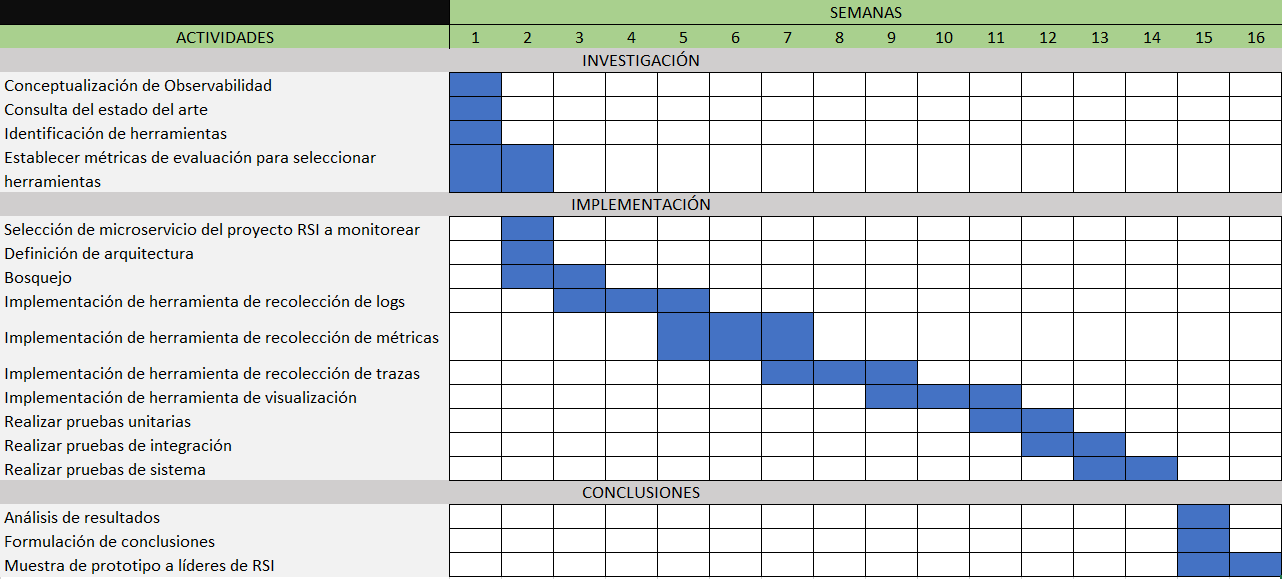
\includegraphics[width=1\textwidth]{images/cronograma-plan.PNG}
    \captionsetup{justification=centering} % Centra el título (caption)
    \caption{Cronograma con las actividades y las semanas.}
    \label{tab:cronograma}
\end{table}														

%%%%%%%%%%%%%%%%%%%%%%%%%%%%
%%%%%%%%%%%%%%%%%%%%%%%%%%%%    PRESUPUESTO
%%%%%%%%%%%%%%%%%%%%%%%%%%%%
\section{\large PRESUPUESTO}

\begin{table}[H]
    \centering
    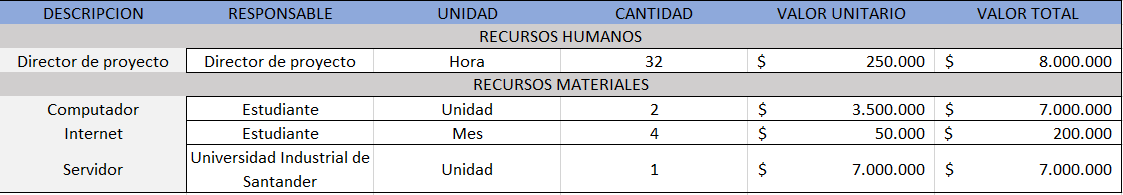
\includegraphics[width=1\textwidth]{images/presupuesto-plan.PNG}
    \captionsetup{justification=centering} % Centra el título (caption)
    \caption{Presupuesto de recursos humanos y materiales.}
    \label{tab:presupuesto}
\end{table}

\newpage
\section{\large BIBLIOGRAFÍA}

\printbibliography


\end{document}

